\chapter{脉冲神经网络}
\par
在过去多年中,人工神经网络(ANN)已能够解决很多问题。但当我们尝试解决更高级的问题时,对算力和电源的不断增长的需求是不可避免的,在可用资源有限的嵌入式系统上几乎不可能采用ANN。
鉴于这些情况,由于事件驱动性和低功率特性,脉冲神经网络(SNN)作为第三代神经网络正在引起广泛关注。然而,SNN的复杂的动态神经元和不可微分的脉冲操作给其带来了显著的性能下降。因此,其应用仅限于相对简单的任务,例如图像分类。
在最近的研究中,Seijoon Kim等人研究了SNN在更具挑战性的对象检测任务中的性能下降\mycite{Spiking-yolo},并提出了第一个用于目标检测的脉冲神经网络模型Spiking-yolo,该模型是对现有的yolo模型进行转化,因此下文中先简述脉冲神经网络的各种学习算法,再重点对转化的方法进行阐述。
\section{学习算法}
\par
人工神经网络的学习是根据数据对网络的关键参数进行调整和优化的过程。
优化学习算法在这一过程中起着至关重要的作用。
目前人工神经网络优化理论中,结合误差反向传播的梯度下降算法是其核心。
\par
相比之下,当前脉冲神经网络领域还没有成熟的训练算法。网络采用的神经元模型和编码方式各异,均造成了训练算法的多样化。
总体来讲,主流的实现SNN的方式有三种:第一种是基于STDP等生物解释性好的算法进行训练,第二种是直接使用BP算法进行反向传播,这实现起来也相对困难。第三种是运用成熟的人工神经网络,对其进行转换,
也可以按是否采用标签信息将其分为无监督学习和有监督学习两类。脉冲神经网络一些常用的学习算法如下图\mycite{2021脉冲神经网络研究进展综述}所示:
\begin{figure}[htbp]
	\centering
	\setlength{\abovecaptionskip}{0cm}  
	\setlength{\belowcaptionskip}{0cm}
	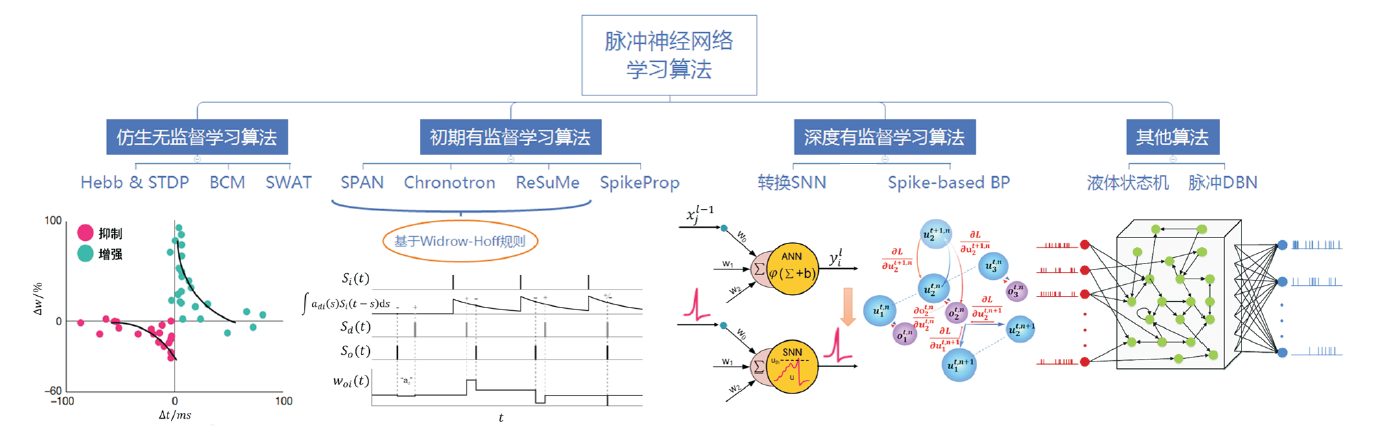
\includegraphics[width=1\textwidth]{figures/study.png}
	\caption{常见的SNN学习算法}
\end{figure}
\section{ANN转化的SNN}
\par
转化SNN (ANN-converted SNN) 是为了在已发展出的深度学习成果上,与硬件结合从而进一步利用事件驱动特性的低能耗优势,从ANN的视角出发的一种SNN实现方法。其作为间接监督性学习算法,
基本理念是在使用ReLU函数的ANN网络中, 用SNN中频率编码下的平均脉冲发放率来近似ANN中的连续激活值。完成原始ANN训练后, 再通过特定的结构将其转换为SNN. 
实质上, 转换SNN的训练依赖的仍是在ANN中进行的反向传播算法, 但是因为没有直接训练SNN的困难. 所以就性能表现而言, 转换SNN保持着与ANN很小的差距, 这一点在大的网络结构和数据集上的良好表现得到了印证\mycite{rueckauer2016theory}。
\subsection{国内外研究进展}
\par
关于ANN-to-SNN转换的早期研究始于\mycitex{2013Conversion}等人的工作。其中CNN单元被取代成具有泄漏和不应期的生物启发的脉冲单元,旨在处理来自基于事件流的输入。\mycitex{Cao2014SpikingDC}等人提出了脉冲神经元传递函数之间的紧密联系,即输入电流和输出发放频率与整流线性单元(ReLU)之间的关系,这是当今人工神经网络中神经元的标准模型。Diehl等人改进了他们的方法。通过使用权重归一化方案,对MNIST\mycite{Lecun}分类任务实现了几乎无损失的人工神经网络转换。该技术重新调整权重以避免由于神经元的过多或过少而导致的SNN中的近似误差。
\mycitex{2016Hun}引入了一种转换方法,其中训练期间的噪声注入通过更逼真的生物神经元模型提高了对SNN的近似误差的鲁棒性。\mycitex{Esser_2016}等演示了一种为TrueNorth平台优化CNN的方法,该平台具有二进制权重和受限连接。\mycitex{zambrano2016fast}开发了一种使用尖峰神经元的转换方法,该神经元适应其环形阈值以减少编码信息所需的尖峰数量。
这些方法在MNIST上取得了非常好的结果,但是当扩展到可以解决CIFAR-10\mycite{Krizhevsky09learningmultiple}的网络时,SNN结果低于最先进的ANN结果。一个原因是,对于提高ANN误差率至关重要的许多运算符的SNN实现(例如最大池化层,softmax激活函数和批量归一化)是不存在的,因此SNN只能近似地匹配ANN的推断。因此,下文中给出一些转化的具体方案和理论知识。
\subsection{脉冲发放率和模拟激活值数学分析}
\par
我们假设ANN单元和SNN神经元之间存在一对一的对应关系,对于具有$L$层的网络,让$\mathbf{W}^l,l \in {1,...,L}$表示连接单元$1-1$至层$l$中的单元的重量矩阵,偏置为$\mathbf{b}^l$。每层中的单元数是$M^l$。层$l$中连续值神经元$i$的ReLU激活计算如下:
\[
a_i^l:= max \Biggl(0,\sum\limits_{j=1}^{M^{l-1}}W_{ij}^la_j^{l-1} + b_i^l \Biggr)
\]\par
每个SNN神经元都具有膜电位$V_i^l(t)$,它在每个时间步长积分其输入电流:
\[
z_i^l(t):= V_{thr} \Biggl(\sum\limits_{j=1}^{M^{l-1}}W_{ij}^l\Theta_{t,j}^{l-1} + b_i^l \Biggr)
\]\par
此处$V_{thr}$是阈值并且$\Theta_{t,j}^{l}$是时间$t$内发放脉冲的阶跃函数
\begin{equation}
	\Theta_{t,j}^{l}= \Theta(V_i^l(t-1) + Z_i^l(t) - V_{thr}),\text{with }
	\Theta(x) = 
	\begin{cases}
		1, & \text{if } x \ge 0; \\
		0, & \text{else.}
	\end{cases}
\end{equation} \par
每个SNN神经元$i$的发放率可以由下计算
\[
\setlength\abovedisplayskip{1pt}
\setlength\belowdisplayskip{1pt}
r_i^l(t):=N_i^l(t)/t
\]\par
其中$N_i^l(t)=\sum_{t'=1}^t\Theta_{t',i}^l$,即脉冲的产生数\par
神经元对输入$z_i^l(t)$进行积分直到膜电势$V_i^l(t)$超过阈值$V_{thr}$,产生脉冲。复位的方式有两种,一种是Diehl等人使用的将膜电势设置为基线,通常为零;另一种是通过减法的复位,在超过阈值时,从膜电势中减去阈值$V_{thr}$。通过减法机制简单地切换到复位可以改善近似,并使转换方案也适用于更深的网络。多余的电荷ǫ在复位时不会被丢弃,可以用于下一个脉冲生成。所以我们优先采用减法重置的方式。\par
对归一化的网络,假定输入恒定为$z \in [0,1]$,对采用减法重置的IF神经元,其膜电势随时间变化为
\[
V_i^l(t) = V_i^l(t-1) + z_i^l(t) -V_{thr}\Theta_{t,i}^l
\]
由前式$Z_i^l = V_{thr}a_i^l$,对T时间步内膜电位进行求和:
\[
\sum\limits_{t=1}^T V_i^l(t) = \sum\limits_{t=1}^T V_i^l(t-1) + z_i^l(t)T - V_{thr}\sum\limits_{t=1}^T\Theta_{t,i}^l
\]\par
移项并且两边同时除$T$
\[
\frac{\sum\limits_{t=1}^T V_i^l(t)-\sum\limits_{t=1}^T V_i^l(t-1)}T = V_{thr}a_i^l - V_{thr}\frac{\sum\limits_{t=1}^T\Theta_{t,i}^l}T
\]
即
\[
r_i^t(t)=a_i^l-\frac{\sum\limits_{t=1}^T V_i^l(t)-\sum\limits_{t=1}^T V_i^l(t-1)}{TV_{thr}}
\]
故在仿真时间步长$T$无限长情况下:
\[
r_i^l(t) = a_i^l(a > 0)
\]
\section{ANN操作的脉冲实现}
\subsection{偏置}
\par
以前提出的SNN转换方法中,因为神经网络的偏置很难表示,所以简单地将其设置为0。在脉冲神经网络中,也可以简单地用比例于偏置的恒定输入流进行表示。 但一些负偏置不得不使用颠倒神经元符号的方式来表示。
\subsection{参数标准化}
\par
Diehl等人引入了权重标准化作为避免由于过低或过高的发放率引起的近似误差的手段。除此之外还有一些其他的归一化方法,在改善转换后SNN的性能
\subsubsection{偏差归一化}
\par
基于数据的权重归一化机制基于ANN的ReLU单元的线性,通过线性地重新调整所有权重和偏差,可以简单地将其扩展到偏差,使得对于所有训练示例,ANN激活a小于1.为了保留层内编码的信息,需要同时缩放一层的参数.将层中的最大ReLU激活表示$\lambda^l=\text{max}[\mathbf{a}^l]$,然后将权重$\mathbf{W}^l$和偏差$\mathbf{b}^l$归一化为$\mathbf{W}^l \to \mathbf{W}^l \frac{\lambda^l}{\lambda^{l-1}}$和$\mathbf{b}^l \to \mathbf{b}^l / \lambda^l$。 

\subsubsection{除异常值归一化}
\par
虽然权重归一化避免了SNN中的发放率饱和,但它可能导致非常低的发放率,从而增加了延迟,直到信息到达更高层。我们将前一段中描述的算法称为“max-norm”,因为归一化因子$\lambda^l$被设置为层内的最大ANN激活,其中使用训练数据的大子集来计算激活。这是一种非常保守的方法,可确保SNN发放率最有可能不超过最大发放率。缺点是该程序易于受到导致非常高的激活的单个异常值样本的影响,而对于大多数剩余样本,该发放率将远低于最大发放率。
\par
因此在实际进行归一化时,我们设置一个百分位数p,称为“归一化标度”,并注意“max-norm”方法在特殊情况p = 100时被恢复。p表现良好的典型值在[99.0,99.999]范围内。引入p的目的就是为了防止除以个别过大的值,导致较低的发放率
\subsection{BN层的转化}
\par
ANN为了快速训练和收敛提出了批归一化(Batch Normalization),批归一化旨在将ANN输出归一化到0均值,这与SNN的特性相违背。因此,需要将BN的参数吸收到前面的参数层中。训练后,这些变换可以整合到权重向量中,从而保留BN的效果,但不需要在推理期间对每个样本重复计算归一化对于给定的网络,这只需要进行一次;在推理期间,参数不会改变。
\par
假定BatchNorm的参数为$\gamma$ (BatchNorm.weight),$\beta$ (BatchNorm.bias),$\mu$ (BatchNorm.mean),$\sigma$ (BatchNorm.var):这四个参数都是在训练期间获得的。参数模块具有参数 $W$ 和 $b$ 。BatchNorm参数吸收就是将BatchNorm的参数通过运算转移到参数模块的 $W$
中,使得数据输入新模块的输出和有BatchNorm时相同。 对此,新模型的$\bar{W}$ 和 $\bar{b}$ 公式表示为:
\[
\bar{W} = \frac{\gamma}{\sigma}W
\]
\[
\bar{b} = \frac{\gamma}{\sigma}(b-\mu) + \beta
\]
\subsection{脉冲层中的最大池化}
\par
大多数\mycite{8594067}成功的人工神经网络使用最大池化来空间下采样特征图。然而,这还没有在SNN中使用。一些现有的方法是基于先到时间脉冲编码,即第一个发放脉冲的神经元被认为是最大的神经元。还有一些简单的脉冲池化机制:输出单元包含门控函数,只允许来自最大神经元的脉冲通过,同时丢弃来自其他神经元的脉冲。